% Change 'digital' to 'printed' before printing
\documentclass[
  digital, %% This option enables the default options for the
           %% digital version of a document. Replace with `printed`
           %% to enable the default options for the printed version
           %% of a document.
  table,   %% Causes the coloring of tables. Replace with `notable`
           %% to restore plain tables.
  lof,     %% Prints the List of Figures. Replace with `nolof` to
           %% hide the List of Figures.
  lot,     %% Prints the List of Tables. Replace with `nolot` to
           %% hide the List of Tables.
  oneside,
  %% More options are listed in the user guide at
  %% <http://mirrors.ctan.org/macros/latex/contrib/fithesis/guide/mu/fi.pdf>.
]{fithesis3}
%% The following section sets up the locales used in the thesis.
\usepackage[resetfonts]{cmap} %% We need to load the T2A font encoding
\usepackage[main=english, slovak]{babel}

%% For non-Latin scripts, it may be necessary to load additional
%% fonts:
\usepackage{paratype}
%%
%% The following section sets up the metadata of the thesis.
\thesissetup{
    date          = 2017/5/22,
    university    = mu,
    faculty       = fi,
    type          = mgr,
    author        = Zuzana Dankovčíková,
    gender        = f,
    advisor       = Bruno Rossi PhD,
    title         = {Custom Roslyn Tool for Real-Time Static Code Analysis},
    TeXtitle      = {Custom Roslyn Tool for Real-Time Static Code Analysis},
    keywords      = {roslyn, C\#, compilers, code review, .NET compiler platform, Kentico, analyzer, code fix...},
    TeXkeywords   = {roslyn, C\#, compilers, code review, .NET compiler platform, Kentico, analyzer, code fix..., \ldots},
}
\thesislong{abstract}{
    TODO: This is the abstract ...
}
\thesislong{thanks}{
    TODO: This is the acknowledgement\dots

}

%% The following section sets up the bibliography.
\usepackage{csquotes}
\usepackage[              %% When typesetting the bibliography, the
  backend=biber,          %% `numeric` style will be used for the
  style=numeric,          %% entries and the `numeric-comp` style
  citestyle=numeric-comp, %% for the references to the entries. The
  sorting=none,           %% entries will be sorted in cite order.
  sortlocale=auto         %% For more unformation about the available
]{biblatex}               %% `style`s and `citestyles`, see:
%% <http://mirrors.ctan.org/macros/latex/contrib/biblatex/doc/biblatex.pdf>.
\addbibresource{mybib.bib} %% The bibliograpic database within
                          %% the file `example.bib` will be used.

\usepackage{makeidx}      %% The `makeidx` package contains
\makeindex                %% helper commands for index typesetting.

%% These additional packages are used within the document:
\usepackage{paralist}
\usepackage{amsmath}
\usepackage{amsthm}
\usepackage{amsfonts}
\usepackage{url}
\usepackage{menukeys}

\begin{document}
% =================================================================
% ============================= CHAPTER 1 =========================
% =================================================================
  \chapter{Introduction}
  [1-2 pages]
  
TODO...

Ideas:

What is code quality, why is it important, tool that support it.. compilers, diversion ... aaaand here comes Roslyn which provides compiler as a platform.  

In~the~.NET world, the~compiler used~to~be a~black box that given the~file paths to~the~source text, produced an~executable. In~order~to do that, compiler has to collect large amount of~information about the~code it is processing. This knowledge, however, was unavailable to~anyone but the~compiler itself and it was immediately forgotten once the~translated output was produced~\cite{roslyn-overview-github}. 

Why is this an~issue when for decades this black-boxes served us well? Programmers are increasingly becoming reliant~upon the~powerful integrated development environments (IDEs). Features like IntelliSense, intelligent rename, refactoring or~"Find all references" are key~to~developers' productivity; and~even more so in~an~enterprise-size systems. 

This gave a~rise to~number of~tools that analyze the~code for common issues and are able to~suggest a~refactoring. The problem is that that such~tool needs to~parse the~code first in~order~to be~able~to~understand and~analyze it. As a result companies need to invest fair amount of resources to duplicate the logic that the .NET compiler already possesses. Not only is it possible that the compiler and the tool may disagree on some specific piece of code, but with every new version of C\# the tool needs to be updated to handle new language features\cite{dot-net-development-using-the-compiler-api}.

With roslyn.. etc. etc. .. API for analysis.. use in companies for custom analyzers... etc. etc....
 https://github.com/dotnet/roslyn/wiki/Roslyn Overview -- motivation
Make sure to stress out that ".NET Compiler Platform" and "Roslyn" names will be used interchangably as it is in Roslyn Succinctly on page 11.


% =================================================================
% ============================= CHAPTER 2 =========================
% =================================================================
  \chapter{Code Quality and Static Code Analysis}
TODO

% =================================================================
% ============================= CHAPTER 3 =========================
% =================================================================
  \chapter{.NET Compiler Platform}
As~per~\cite{dragon-book}, compiler is a~program that can read a~program in a~\textit{source} language and~translate it into a~semantically equivalent program in~a~\textit{target} language while reporting any errors detected in~the~translation process. 

In~the~.NET world, the~compiler used~to~be a~black box that given the~file paths to~the~source text, produced an~executable. This perception was changed in~2015 when Microsoft introduced the .NET Compiler Platform (commonly referred to as "Project Roslyn").  

%\begin{figure}[h!]
%		\centering
%			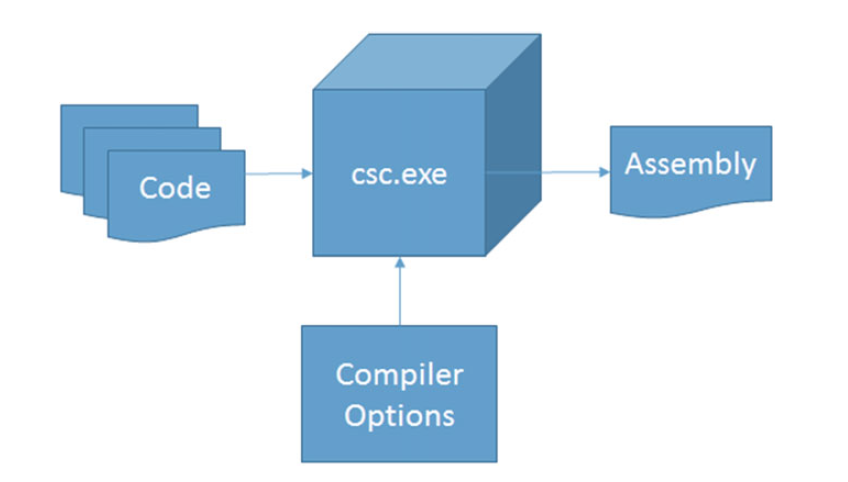
\includegraphics[scale=0.35]{img/compiler-as-a-black-box}
%		\caption{Compiler as a black box~\cite{dot-net-development-using-the-compiler-api}}
%		\label{fig:compiler-as-a-black-box}
%\end{figure}

Not only have been compilers for both Visual Basic and C\# rewritten into the entirely managed code, they also expose the internals of the compiler pipeline via a public .NET API~\footnote{Application Programming Interface}. This makes them a platform (also known as \textit{compiler-as-as-service}) with rich code analysis APIs that can be leveraged by developers to perform analysis, code generation or dynamic compilation in their own programs~\cite{roslyn-succinctly}. Those can be then easily integrated into the Visual Studio all without the hard work of duplicating compilers' parsing logic.

This chapter will take a look at how the Roslyn API layers are structured, how the original source code is represented by the compiler and how developers can build tools upon the compiler's API. Lastly it will provide a short overview and evaluation of other tools that were used before Roslyn or have emerged thanks to .NET Compiler Platform.

Note that although Roslyn provides equivalent APIs for both VisualBasic and C\#, this thesis will only focus on the latter since only that one is relevant for the practical part of the thesis.  
  
  \section{The Compiler Pipeline}
Roslyn compilers expose an API layer that mirrors the traditional compiler pipeline (see \ref{fig:roslyn-compiler-pipeline}). However, instead of a single process of generating the target program, each compilation step is treated as a separate component~\cite{roslyn-overview}:

\begin{itemize}
  \item \textbf{Parse phase} consists of \textit{lexical analysis} (\textit{scanner}) and \textit{syntactic analysis} (\textit{parser}). First, the lexical analyzer processes the stream of characters from the source program and groups them into meaningful sequences called \textit{lexemes}. Those are subsequently processed by the \textit{syntax analyzer} that creates a tree-like structure of tokens based on the language's grammar~\cite{dragon-book}.

  \item \textbf{Symbols and metadata phase} where named symbols are generated based on the declarations from the source and imported metadata.

  \item \textbf{Bind phase} in which the identifiers from the source code are matched to their respective symbols.

  \item \textbf{Emit phase} where all the gathered information is used to emmit an assembly.
\end{itemize}

\begin{figure}[h!]
		\centering
			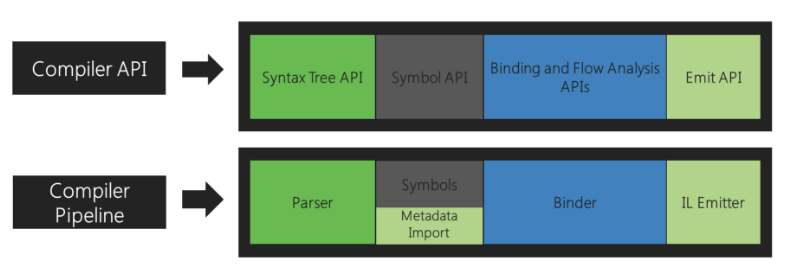
\includegraphics[scale=0.5]{img/roslyn-compiler-pipeline}
		\caption{Compiler pipeline~\cite{roslyn-overview}}
		\label{fig:roslyn-compiler-pipeline}
\end{figure}

In each phase, the .NET Compiler Platform creates an object model containing gathered information and exposes it through the API in form of .NET objects. These object are also used internally by Visual Studio~\footnote{The new generation of Visual Stuio leveraging from the Roslyn compiler are called vNext and first one was VS 2015.} to support basic IDE functionality. For instance \textbf{syntax tree}, that is the result of the parse phase, is used to support formatting and colorizing the code in the editor. The result of the second phase -- \textbf{hierarchical symbol table}, is the basis for \textit{Object browser} and \textit{Navigate~to} functionality. Binding phase is represented as an \textbf{object model that exposes the result of the semantic analysis} and is utilized in \textit{Find all~references} or \textit{Go~to~definition}. Finally, the Emit phase produces the~Intermediate Language (IL) byte codes and is also used for \textit{Edit and~Continue} feature~\cite{roslyn-overview}.

  \section{The .NET Compiler Platform's Architecture}
The Roslyn's architecture consists of two main layers - Compiler and Workspaces APIs, and one secondary layer - Features API, as seen on Figure~\ref{fig:roslyn-compiler-architecture}.

\begin{figure}[h!]
		\centering
			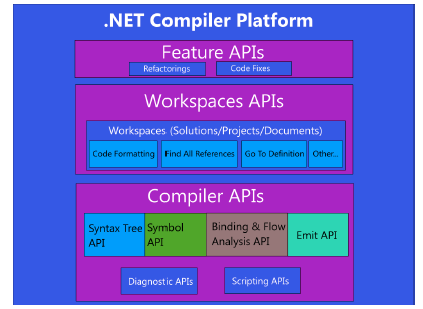
\includegraphics[scale=0.6]{img/roslyn-compiler-architecture}
		\caption{.NET Compiler Platform Architecture~\cite{roslyn-succincly}}
		\label{fig:roslyn-compiler-architecture}
\end{figure}

One of the key concepts of .NET Compiler Platform is immutability. The compiler exposes hundreds of types that represent all information about source code from \texttt{Project} and \texttt{Document} to \texttt{SyntaxTrees} with almost all of those types being immutable. This means, that once created, the object cannot change. In order to alter it in any way, new instance must be created, either manually, or from an existing instance by applying one of many \texttt{With()} methods that the API provides.

The immutability enables the compiler to perform parallel work without need to create duplicate objects or apply any locks on them. This concept is useful for the command line compiler but it is considered extremely important for IDEs where it enables for one document to be handled by multiple analyzers in parallel.

  \subsection{The Compiler APIs}
As discussed in the previous section, the Compiler APIs offer an object model representing the results of syntactic and semantic analysis produced by the respective phases of the compiler pipeline. Moreover, it also includes an immutable snapshot of a single compiler invocation, along with assembly references, compiler options, and source files. This layer is agnostic of any Visual Studio components and as such can be used in stand-alone applications as well. There are two separate, though very similar, APIs for Visual Basic and C\#, each providing functionality tailored for specific language nuances.

  \subsubsection{Diagnostic APIs}
Apart from parsing code and producing an assembly, the compiler is also capable of raising diagnostics, covering everything from syntax to semantics, and report them as errors, warnings or information messages~\cite{roslyn-succinctly}. This is achieved through the compilers' Diagnostics APIs that allow developers to effectively plug-in to compiler pipeline, analyze the source code using the exposed object models, and surface custom diagnostics along with those defined by the compiler itself. These APIs are integrated to both MSBuild~\footnote{The Microsoft Build Engine https://github.com/Microsoft/msbuild} and Visual Studio (2015 and newer). providing seamless developer experience. The practical part of this thesis relies on Diagnostic APIs to provide custom diagnostics and the details will be discussed in Chapter \ref{chap:custom-roslyn-analyzers}.

  \subsubsection{Scripting APIs}
As a part of the compiler layer, Microsoft team has introduced new Scripting APIs that can be used for executing code snippets. These APIs were not shipped with .NET Compiler Platform 1.0 and are part of v2.0.0 RC3\footnote{Release candidate 3, as per https://github.com/dotnet/roslyn/wiki/Scripting-API-Samples [26-02-2017].}.

  \subsection{Workspaces APIs}
Workspace represents a collection of solutions, projects, and documents. It provides a single object model containing information about the projects in a solution and their respective documents; exposes all configuration options, assembly and inter-project dependencies, and provides access to syntax trees and semantic models. It is a starting point for performing code analysis and refactorings over entire solutions.

Although it is possible to use the \texttt{Workspace} outside of any host environment, the most common use case is an IDE providing an instance of \texttt{Workspace} that corresponds to the open solution. Since the instances of \texttt{Solution} are immutable, the host environment must react to every event (such as user key stroke) with an update of the \texttt{CurrentSolution} property of the \texttt{Workspace}.

  \subsection{Feature APIs}
This layer relies on both compiler and workspaces layers and is designed to provide API for offering code fixes and refactorings. This layer was also used while working on the practical part of this thesis.
  
  \section{Syntax Tree}
As mentioned in the previous sections, the product of the syntactic analysis is a syntax tree. It enables developers to work with the code in a managed way instead of working against plain text. Syntax trees are used for both analysis and refactorings, where the new code is generated either manually or as a modified version of the existing tree. While being immutable, syntax trees are thread-safe and analysis can be done in parallel.

It is important to point out, that in a same way the compiler constructs a syntax tree from the source text, it is also possible to round-trip back to the text representation. Thus, the source information is always preserved in full fidelity. This means that every piece of information from source must be stored somewhere within the tree, including comments, whitespaces or end-of-line characters. 

Figure~\ref{fig:roslyn-syntax-tree} shows a syntax tree of an invocation expression as obtained from Syntax Visualizer\footnote{https://roslyn.codeplex.com/wikipage?title=Syntax\%20Visualizer} extension available in Visual Studio. This tool is useful for understanding how Roslyn represents particular language constructs and is widely utilized whenever one needs to analyze the code. Following sections explain what are the main building blocks of such syntax tree and will refer to this figure:

\begin{figure}[h!]
		\centering
			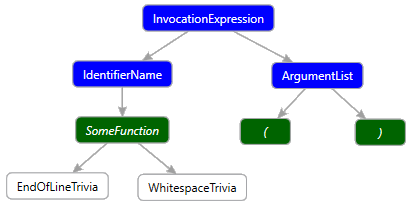
\includegraphics[scale=0.8]{img/roslyn-syntax-tree-2}
		\caption{Syntax tree of an invocation expression}
		\label{fig:roslyn-syntax-tree}
\end{figure}

  \subsubsection{Syntax Nodes}
Syntax nodes (blue color) are non-terminal nodes of a syntax tree, meaning they always have at least one other node or token as a child. Nodes represent syntactic constructs of a language such as statements, clauses or declarations. Each type of node is represented by a single class deriving from \texttt{SyntaxNode}. Apart from common properties \texttt{Parent}, \texttt{ChildNodes} and utility methods like \texttt{DescendantNodes}, \texttt{DescendantTokens}, or \texttt{DescendantTrivia}, each subclass exposes specific methods and properties. As shown in Figure~\ref{fig:roslyn-syntax-tree}, \texttt{InvocationExpression} has two properties, \texttt{IdentifierName} and \texttt{ArgumentList} both of which are \texttt{SyntaxNodes} themselves.
 
  \subsubsection{Syntax Tokens}
As opposed to nodes, syntax token (green color) represent terminals of the language grammar, such as keywords, punctuation, literals and identifiers. For the sake of efficiency, \texttt{SyntaxToken} is implemented as a value type (C\# structure) and there is only one for all kinds of tokens. To be able to tell them apart, tokens have \texttt{Kind} property. For example, \texttt{SomeFunction} is of kind \texttt{IdentifierName}, whereas "\texttt{(}" character is \texttt{OpenParenToken}.

  \subsubsection{Syntax Trivia}
In order to enable refactoring features, syntax trees must also store information about whitespaces, comments and preprocessor directives that are insignificant for compilation process itself. This information is represented by another value type -- \texttt{SyntaxTrivia} (white color). Trivia are not really parts of the tree itself, rather they are properties of tokens accessible by their \texttt{LeadingTrivia} and \texttt{TrailingTrivia} collections.

  \section{Semantics of the Program}
% Start with why semnatics is important in addition to syntax - some cool stuff from dragonbook. Tell about symbol tables in all compilers. Talk about ISymbol in Roslyn. Mention Compilation and wrap it up with Sematic model.

Even though syntax trees are enough to describe proper form of the program (compliance to the language grammar), they cannot enforce all language rules, for example, type checking. In order to tell whether a method is called with the right number of arguments, or operator is applied to operands or right type, it's inevitable to introduce semantics. 

As described in~\cite{dragon-book}, one of the core responsibilities of a compiler is to collect information about all elements and their properties from the source program. These are attributes such as identifier name, type, allocated storage, scope or for method names the number and types of arguments and their return values.

All this data is being incrementally collected when parsing the source code (analysis phase) and is stored in \textit{symbol tables}. These are later used in synthesis where intermediate language representation is produced.

  \subsubsection{Symbols}
In .NET Compiler Platform, a single entry of a symbol table is represented by a class deriving from \texttt{ISymbol}. The symbol represents every distinct element (namespace, type, field, property, event, method or parameter) either declared in the source code or imported as metadata from a referenced assembly. Each specific symbol has its own methods and properties often directly referring to other symbols. For example \texttt{IMethodSymbol} has a \texttt{ReturnType} property specifying what is the type symbol the method returns.

  \subsubsection{Compilation}
An important immutable type, that represents everything needed to compile a C\# (or Visual Basic) program is a \texttt{Compilation}. It contains all source files, compiler options and assembly references. Compilation provides convenient ways to access any discovered symbol. For instance, it is possible to access the entire hierarchical symbol table rooted by global namespace or look up type symbols by their common metadata names.

  \subsubsection{Semantic Model}
When analyzing a single source file of a compilation, all its semantic information is available through a \textit{semantic model}. The \texttt{SmeanticModel} object can answer many questions such as:
  \begin{itemize}
  \item What symbol is declared at the specific location in the source?
  \item What is the result type of an expression?
  \item What symbols are visible from this location?
  \item What diagnostics are reported in the document?
  \end{itemize}
 
This makes semantic model very useful when performing static code analysis concerned with more than just syntax.
 
  \pagebreak
  \section{Analysers and Code Refactorings}
  [3 pages?]
  
%  - how to perform static code analysis with Roslyn
%    - writing anlyzers and code fixes / code refactorings  
  
  \pagebreak 
  \section{Other Tools}
  [2-3 pages?]
TODO: Should this be a separate chapter????

  3. Other tools for code analysis available for C\#
  
  - new DotNetAnalyzers available thanks to Roslyn

  - Resharper,
  
  - FxCop

  - StyleCop

% =================================================================
% ============================= CHAPTER 4 =========================
% =================================================================
\chapter{Kentico CMS Internal Guidelines}
[3-4 pages]

What is Kentico CSM?

Current situation \& motivation

- how code reviews are done at kentico

- tools that aid code reviews (??)

  - original BugHunter

  - use of FxCop and ReSharper
  
% =================================================================
% ============================= CHAPTER 5 =========================
% =================================================================
\chapter{Implementation of Custom Analyzers}
\label{chap:custom-roslyn-analyzers}
[5-7 pages]

How was the tool implemented, 

Project structure,

What it contains

Concerns about Performance

% =================================================================
% ============================= CHAPTER 6 =========================
% =================================================================
\chapter{Measuring and Optimizing the Performance}
[up to 7 pages?]

Why tool needs to be super-fast (refer to chapter 4 where this should have been said)

Talk about /ReportAnalyzer switch of MSBuild process (csc.exe)

How the performance of the slowest analyzers (SystemIO, BaseChecks) was improved

Talk about how analyzers deployment influenced the build time

Questionares sent to development team, feedback from senior developers

% =================================================================
% ============================= CHAPTER 7 =========================
% =================================================================
\chapter{Deployment and Versioning}
[2 pages]

% =================================================================
% ============================= CHAPTER 8 =========================
% =================================================================
\chapter{Conclusion}
[1-2 pages]

% =================================================================
% =============================== STUFF ===========================
% =================================================================
	% From template
	\makeatletter\thesis@blocks@clear\makeatother
	\phantomsection %% Print the index and insert it into the
	\addcontentsline{toc}{chapter}{\indexname} %% table of contents.

	\printindex
    
% =================================================================
% =========================== BIBLIOGRAPHY ========================
% =================================================================
    \printbibliography

% =================================================================
% ============================ APPENDICES =========================
% =================================================================    
	\appendix %% Start the appendices.
  \chapter{Questionnaires}
TODO...

\end{document}
